% Created 2021-02-17 Wed 12:06
% Intended LaTeX compiler: pdflatex
\documentclass[a4paper]{article}
\usepackage[utf8]{inputenc}
\usepackage[T1]{fontenc}
\usepackage{graphicx}
\usepackage{grffile}
\usepackage{longtable}
\usepackage{wrapfig}
\usepackage{rotating}
\usepackage[normalem]{ulem}
\usepackage{amsmath}
\usepackage{textcomp}
\usepackage{amssymb}
\usepackage{capt-of}
\usepackage{hyperref}
\usepackage{listingsutf8}
\usepackage{minted}
\usepackage[margin=0.5in]{geometry}
\usepackage{parskip}
\usepackage[cache=false]{minted}[obeytabs]
\newcommand{\sh}[1]{\lstset{language={Bash},basicstyle={\ttfamily\small}}\lstinline{#1}}
\usemintedstyle{emacs}
\newminted{common-lisp}{fontsize=\footnotesize}
\author{Marco Hassan}
\date{\today}
\title{Emacs Hands On Session - Some Libraries}
\hypersetup{
 pdfauthor={Marco Hassan},
 pdftitle={Emacs Hands On Session - Some Libraries},
 pdfkeywords={},
 pdfsubject={},
 pdfcreator={Emacs 27.1.91 (Org mode 9.4.4)}, 
 pdflang={English}}
\begin{document}

\maketitle
\tableofcontents

\setlength\parindent{0pt}


\section{After Installation}
\label{sec:org05d234a}

Notice that after the installation your Emacs will not look like
mine. It will be an ugly white program with little functionality.

\begin{center}
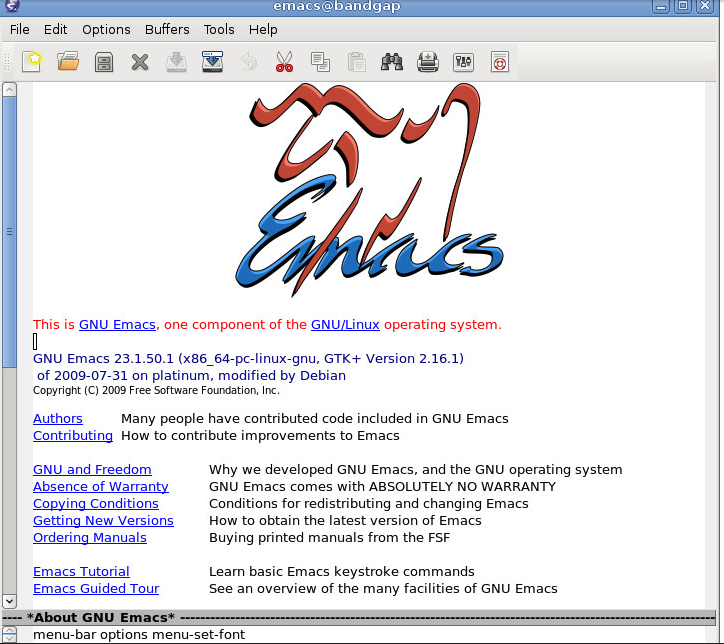
\includegraphics[width=.9\linewidth]{images/Bildschirmfoto 2021-02-17 um 10.52.06.png}
\end{center}

The key idea is the \textbf{customization} idea of Emacs that we previously
discussed.

Emacs is shipped as almost nothing at the beginning - i.e. all of
the cool packages are not included. It is up to you to make sense of
it and customize your emacs however you want.

To do that you have essentially to modify your \texttt{.emacs} file. This
is usually in the \texttt{\textasciitilde{}} folder. If it does not exists create it.

You also will have an \texttt{.emacs.d} directory in the \texttt{\textasciitilde{}} where all of the
downloaded packages will live. If it does not exists create it.

Then enable all of the different package managers. MELPA, Marmalade,
ELPA, mirrors etc.

You are good to go and start to download the packages you
want. Check at the \texttt{M-x list-packages} function.


\section{Other Way - Centaur and possibly similar}
\label{sec:orgde39d54}

The other way is not to download emacs from the official
source and start from scratch at your speed.

There are people that went extremely harsh into emacs and created
crazy emacs configurations.

They dockerized everything such that you should theoretically be
able to run the docker image for such emacs, with all of the
dependencies on the 1000s packages you will use next to your emacs.

You will then be blown at the beginning with a crazy out of the box
emacs. I know one such option is centaur emacs. You can find \href{https://github.com/danielcnorris/centaur-emacs}{it
here}.

I have no experience with it. I started two years ago with emacs and
coming from economics I had no great idea of the software world. I
started from 0 and by googling made my way. Might be that this is a
very viable option. I will not switch as everything I have of my
emacs comes from me and I know my emacs like my pockets.

This is the decision you will have to make. If you go with centaur
and similar it might be tough to jump in such a huge sea without
having any clue on how to navigate it. Maybe it is better to go
slower but build your own emacs where you understand all of the
config and all what you have in there.

You can then spend time, from time to time to check what others are
doing. I choose this road, coping from here and there but always
integrating everything myself such that I know what it is in my
emacs. Up to you there is no right or wrong.


\section{My Emacs Configuration and some Packages I like}
\label{sec:orge2057b7}

\subsection{Task Management and Agenda}
\label{sec:org08dd819}

\subsubsection{Have a word on Org-Mode}
\label{sec:org0fbfa94}
\subsubsection{Explain the task management}
\label{sec:org0d8dedf}
\subsubsection{Explain how you can view todos - for one file or project}
\label{sec:orgdba07ee}
\subsubsection{Explain how you can decide what tasks status you can cycle with}
\label{sec:org470a10a}
\subsubsection{Show the org capture}
\label{sec:org55cd71e}
\subsubsection{Show agenda}
\label{sec:orge4bd6ff}
\subsubsection{Recall the org journal some people work with it}
\label{sec:org01c1641}

I  personally never took the time to check at this into detail
\subsubsection{Talk about tags}
\label{sec:orge495ac9}


\subsection{Org babel and literate Programming}
\label{sec:org6a1802a}
Notice this is the best for product documentation or for projects
where you have total ownership of something. As soon as you start
to work in big projects of course there are limits to the extent to
which you can use it. As soon as you tangle you tangle it all and
overwrite the buffer.

I do not know, and did not check to this point if there is some
conflict resolution scheme similar to git that you can
integrate. That would be the endgame.

Also for working and learning by your own this is great.

\subsubsection{Python - Example}
\label{sec:orgec46910}

Hello I write my documentation here. I do literate
programming. Write what I am doing both for myself and for the
friends I have to work with such that they will love me.

\begin{minted}[frame=lines,linenos=true]{python}
print ("Hello world")    
\end{minted}

Above I have written hello world. Next I will write this very
complex function that is key to my project.

\begin{minted}[frame=lines,linenos=true]{python}
def win_1mio ():
    return 10**6
\end{minted}

Etc. etc. You got the idea.

Notice that through the session argument above babel understand
that all of the blocks in the subtree belongs to the same runtime

\begin{minted}[frame=lines,linenos=true]{python}
a = 2
\end{minted}

\begin{minted}[frame=lines,linenos=true]{python}
a
\end{minted}

\subsubsection{Tell that this is just a dummy and fraction of possibilities}
\label{sec:org5a35e17}

\subsubsection{Can pipe results from one org block to another; mix languages and much more}
\label{sec:org5b0ee26}

\subsubsection{On Compiler - based Languages}
\label{sec:org77e8129}

Also other languages work. Even languages that need a compiler!
Did not use this myself and have no idea how the workflow for such
languages is but I know for sure that experts Software Engineers
and Developers use it - so you might want to check online if that
is anything interesting for your.



\subsection{PlatUML - For Architects / Software Engineers}
\label{sec:org51945cb}

\subsubsection{Show this dummy example}
\label{sec:orgbc6e6a5}

Once you set it up you can create your UML diagrams directly into
Emacs. You can check at the \href{https://plantuml.com/de/}{PlantUML documentation}.

Example:

\begin{minted}[frame=lines,linenos=true]{plantuml}
   @startuml
   package "Some Group" {
     HTTP - [First Component]
     [Another Component]
   }

   node "Other Groups" {
     FTP - [Second Component]
     [First Component] --> FTP
   }

   cloud {
     [Example 1]
   }


   database "MySql" {
     folder "This is my folder" {
       [Folder 3]
     }
     frame "Foo" {
       [Frame 4]
     }
   }


   [Another Component] --> [Example 1]
   [Example 1] --> [Folder 3]
   [Folder 3] --> [Frame 4]
      circle A
      circle B
      circle C
      circle D


      A --> B
      A --> C

      B --> D
      C --> D
   @enduml
\end{minted}

\begin{center}
\includesvg[width=.9\linewidth]{/Users/marcohassan/Desktop/emacs_presentation/Hands_On/images/uml_example}
\end{center}


\subsection{Scientific Documentation}
\label{sec:orge02bc25}

\subsubsection{Show Export in Latex}
\label{sec:orge5d9063}

\subsubsection{Show Export in HTML}
\label{sec:org143539c}


\subsection{Ein - Emacs Jupyter Notebook}
\label{sec:orgbcb0dbd}
Show then how you can program in emacs and how also all the
matplotlib stuff.

\subsection{Magit}
\label{sec:orge3da19e}

\subsubsection{Show magit Example}
\label{sec:org6a27536}


\section{Warning}
\label{sec:orgdcb5400}

You live in your own bubble once you start with emacs. Consider it
well if that is something you want to do. There are plenty of other
workflow options. This is a rather complex and involved one.

I hope that I made some of the advantages clear. Notice that on the
downside is that it is something that you have to invest lots of
time in. Continuously. Software evolves and so does your emacs.

I learned it when I was not working and just studying during my
Masters and had quite a bit of spare time.

I love it and now that I did the effort will never go back. The
majority of the people around you will not understand what you are
doing with your emacs and so you will not be appreciated for being
an emacs master by itself.

You have to do it for your own and because you believe that with it
you can reach a higher productivity. And this is why eventually
people will appreciate you at work even if they have no clue about
why your screen always looks like you are still in the 90s.
\end{document}
